% ============================================================
%  Chapter fragment -- included by main.tex
%  (not a standalone document; compile main.tex to build the PDF)
% ============================================================
\begin{multicols*}{3}
\raggedcolumns

\sheettitle{03 -- Security Controls: SIEM}{SWS2 -- ZHAW / Tellenbach}

% ==================== SECURITY CONTROLS REVISITED ====================
\section{Detecting a Security Problem}

\subsection{The data problem}
Controls (firewalls, AV, IDS, vuln scanners...) all \kw{produce data}:
\begin{itemize}
\item \kw{Preventive} controls $\to$ data on an attack that \kw{failed} (e.g. login).
\item \kw{Detective} controls $\to$ data on an attack \kw{just happening} (e.g. IDS).
\item \kw{Corrective} controls $\to$ data on \kw{corrective actions} (e.g. DDoS offloading).
\end{itemize}
Volume: mid-size co. = \kw{millions of events/day}; large co. = \kw{billions/day}; netflow huge.
$\Rightarrow$ \hl{information overload}: find THE \kw{needle in a stack of needles}.

\subsection{Two challenges $\to$ two tools}
\begin{itemize}
\item 1st: \kw{Log management} (have \& handle the logs).
\item 2nd: \kw{Make sense} of security-relevant log data.
\item Both addressed by a \kw{SIEM} (or separate log mgmt + SIEM).
\end{itemize}

% ==================== LOG MANAGEMENT ====================
\section{Log Management}

\subsection{Before making sense of logs}
\begin{itemize}
\item You need to \kw{have logs}! Solidify the \kw{logging process}: what is logged where/why, how long \& where stored.
\item Consider \kw{legal aspects} -- behavioural tracking can be problematic.
\end{itemize}
Solutions help with: \kw{collection, retention, indexing/parsing \& searching, reporting} (all log types). \textit{Tools: Logstash, Graylog, Splunk, AlienVault, LogRhythm.}

\subsection{Architecture (3 tiers)}
\begin{itemize}
\item \kw{1 Log generation}: hosts/services/apps that create logs.
\item \kw{2 Log analysis + storage}: log servers receive/copy logs from tier 1.
\item \kw{3 Log monitoring}: dashboards to review data + automated-analysis results.
\end{itemize}
Real-time, near-real-time or batched; today often \kw{scalable cloud} architectures.

% ==================== SIEM ====================
\section{SIEM}

\subsection{What it does}
\kw{Security Information \& Event Management}: gathering, aggregating, \kw{correlating}, analysing, \kw{prioritizing} \& presenting info from \kw{disparate systems}. The "\kw{E}" = correlates \kw{events}, raises \& prioritizes alerts.
\textit{Funnel:} 3M total events $\to$ 15k correlated $\to$ 24 high-prio alarms $\to$ \kw{8 true incidents}.

\subsection{Usage scenarios}
\begin{itemize}
\item \kw{SOC}: analysts 24/7, chase alerts.
\item \kw{Mini-SOC} / "morning after": 1/24, review \& drill down.
\item \kw{Automated SOC}: configure \& forget, alerts only.
\item \kw{Compliance reporting}: review weekly/monthly.
\end{itemize}
Stealthy/advanced attacks $\Rightarrow$ SIEM must learn what's \kw{normal (baseline)} \& flag the \kw{exceptions (anomalies)}.

\subsection{Architecture \& key components}
Sources $\to$ \kw{Collectors} $\to$ \kw{Normalize} (common format) $\to$ \kw{Correlation Engine} + data repo $\to$ Dashboard/Alerts/Reports $\to$ \kw{SOC}.
\textit{Commercial: IBM QRadar, HP ArcSight, Splunk. Open-source: AlienVault OSSIM, Wazuh, SIEMonster.}
\begin{itemize}
\item \kw{Asset directory}: asset value for \kw{risk calc/prioritization}.
\item \kw{Vulnerability scanner}: correlate host alerts with its known vulns.
\item Sources: firewall/auth/system logs, availability monitoring, AV, honeypots, \kw{HIDS/NIDS}.
\end{itemize}

\begin{center}
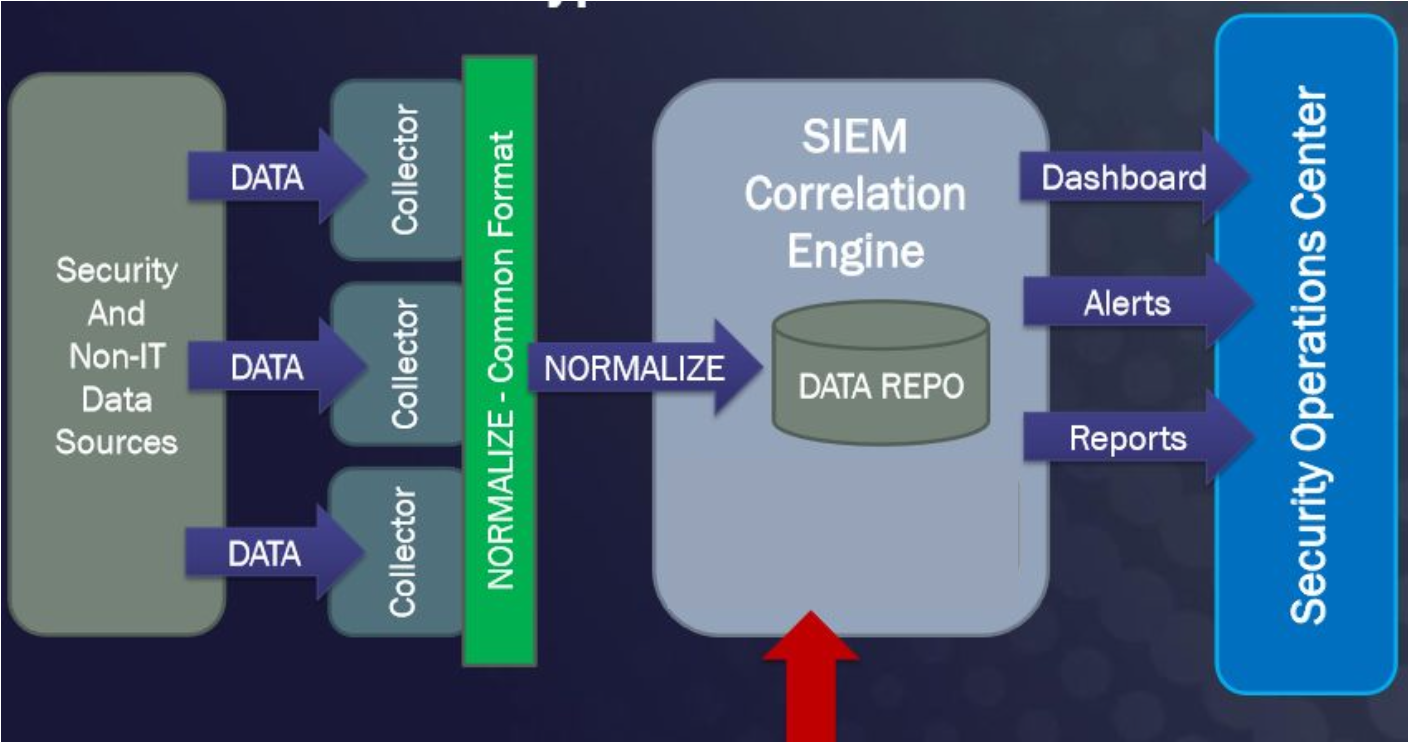
\includegraphics[width=\linewidth]{Figures/siem_architecture.png}
\end{center}

% ==================== IDS / IPS ====================
\section{IDS / IPS}

Intrusion Detection System (IDS) vs Intrusion Prevention System (IPS)

\subsection{IDS vs IPS}
\begin{itemize}
\item \kw{IDS}: monitors network/system activity to \kw{detect} attacks \& abuse (detect + log only).
\item \kw{IPS}: adds a component to \kw{prevent/mitigate} the detected attack.
\item IPS risk: a \kw{false positive} can \kw{lock out legitimate users} (e.g. block a customer); some damage may already be done by detection time.
\item Two types: \kw{Host-based} (HIDS/HIPS) \& \kw{Network-based} (NIDS/NIPS).
\item Components: host/network \kw{sensors}, central DB, \kw{correlation engine}, mgmt console.
\end{itemize}

\subsection{HIDS / HIPS}
\begin{itemize}
\item \kw{HIDS}: sensor software \kw{on the monitored host}; watches system calls, app logs, file modifications, processes, host network data. \textit{Ex: OSSEC, AIDE, Samhain, Fail2Ban, Sagan.}
\item \kw{HIPS} actions: quarantine files, restore from storage, suspend accounts, update firewall (block IP), start/kill processes, shut down.
\item \textit{Ex: \kw{Fail2Ban}} -- scans logs (e.g. apache error\_log), detects malicious IPs (too many failed logins / probing), updates firewall to reject IP for a time.
\end{itemize}

\subsection{NIDS / NIPS}
\begin{itemize}
\item \kw{NIDS}: sensors are \kw{devices in the network} seeing the traffic (switch monitor port, network tap, security gateway); analyses traffic for malicious/suspicious activity. \textit{Ex: Snort, Bro, Suricata, Sagan.}
\item \kw{NIPS}: traffic must \kw{flow through} a monitor/block component. On event: traffic blocked temporarily $\to$ rule engine decides alert; no alert = forward, alert = block (log \& discard).
\end{itemize}

\subsection{Suricata rule (example)}
{\scriptsize\texttt{alert tcp \$EXTERNAL\_NET any -> 10.200.0.0/24 80 (msg:"...root.exe access"; ...; sid:1255;)}}
\begin{itemize}
\item \kw{\$EXTERNAL\_NET}: all IPs not in \$HOME\_NET.
\item \kw{\$HOME\_NET}: user-defined ranges (default 192.168/16, 10/8, 172.16/12).
\item \kw{any}: from any source port; \kw{->} = connection to.
\item \kw{msg}: text shown in the logged alert.
\end{itemize}

\subsection{Measuring IDS performance \hl{(!)}}

\kw{FPR} = FP/(FP+TN) -- "ratio of \kw{benign} points classified as attack".
\kw{FNR} = FN/(FN+TP) -- "ratio of \kw{attack} points classified as benign". benign = gutartig

\kw{Precision} (= "alert quality", slide calls it TPR) = TP/(TP+FP) = how often an alert is a \kw{real} attack.
\textit{Marketing: FPR 0.1\%, FNR 0\% (misses no attack) -- sounds great!}

\textbf{Ex (Scenario 1)} -- 500k pts/day, 0.1\% are attacks. \hl{Two different 0.1\% on two pools:}
\begin{itemize}
\item \kw{TP = 500} = 0.1\% of \kw{all} 500k = the \kw{real attacks} (all caught, FNR 0).
\item \kw{FP $\approx$ 499} = FPR 0.1\% of the \kw{499.5k benign} pool = \kw{false alarms}.
\item Alerts = TP+FP = 999 $\to$ precision = 500/999 $\approx$ \kw{50\%} are real.
\end{itemize}
\kw{Scenario 2}: 10M pts/day, 0.006\% attacks $\to$ TP=600, FP$\approx$9999 $\to$ precision $\approx$ \kw{5.6\%}.
$\Rightarrow$ \hl{False Positive Paradox / base-rate fallacy}: attacks are \kw{rare}, so a tiny FPR on the \kw{huge benign pool} produces $\geq$ as many false alarms as real attacks. When \kw{attack rate $<$ FPR}, FPs dominate. A "99.9\% accurate" IDS can still give mostly junk alerts.

\subsection{Strengths \& limitations}
\begin{itemize}
\item \kw{+} detects known patterns (SQLi, scans, malware spread, anomalies); IPS stops attacks.
\item \kw{-} must be \kw{tuned} for low FPR/FNR; NIDS \kw{can't see encrypted} traffic; IDS doesn't stop attacks (needs humans); IPS must buffer/delay packets (resource-heavy, limits correlation); IPS FPs lock out users.
\end{itemize}

% ==================== EVENT CORRELATION ====================
\section{Event Correlation}

\subsection{Concept}
"\kw{Establish relationships between events}": combine multiple isolated events into \kw{one relevant incident} -- "if this, followed by that, take action". \textit{Ex: Nessus finds Heartbleed on host X, then IDS alerts suspected Heartbleed attack $\Rightarrow$ raise alert.}
Compares parameters: src/dst IP, user/machine, time. \kw{Not} reliant on a single signature/rule $\Rightarrow$ powerful attack-pattern analysis from \kw{multiple independent inputs}.

\subsection{Baseline \& anomaly \hl{(!)}}
\kw{Baseline} = what is normal; \kw{anomaly} = exception. \textit{Ex: Sally (financial analyst) logs into AD Mo--Fr 08:30--08:39; suddenly SSH to DNS server + logins at 01:31/06:02 weekend $\Rightarrow$ anomaly.} \textit{Ex: badge "exit building" 16:00, then login to perimeter server 16:02 $\Rightarrow$ impossible.} $\Rightarrow$ correlation + \hl{clean baselines} are vital.

\subsection{AlienVault SIEM processing}
Normalized events $\to$ evaluated against \kw{policies} (= conditions + consequences):
\begin{itemize}
\item \kw{Conditions}: which events a policy processes.
\item \kw{Consequences}: what happens (send email, forward/modify/create/drop event, alter priority/reliability).
\end{itemize}

\subsection{Risk assessment formula \hl{(!)}}
\kw{risk = asset $\times$ (reliability $\times$ priority / 25)}
\begin{itemize}
\item \kw{Asset value} 0--5 (asset importance).
\item \kw{Priority} 0--5 (based on event type).
\item \kw{Reliability} 0--10 (is it really an attack?).
\item \hl{Alarm if risk $\geq$ 1}. Higher risk = examine first.
\end{itemize}
Vuln scans (OpenVAS) become event sources; severity $\to$ reliability.

\subsection{Correlation vs Cross-correlation}
\begin{itemize}
\item \kw{Correlation}: rules associate multiple events from the \kw{same data source}. \textit{Ex: brute-force = correlate failed + successful logins from same IP; rising reliability with count; limit to bad-reputation hosts.}
\item \kw{Cross-correlation}: events from \kw{different data sources}. \textit{Ex: correlate IDS alert with vuln info $\to$ if target is vulnerable, set reliability to max.}
\end{itemize}

% ==================== USE CASES ====================
\section{(Threat) Use Cases}

\subsection{What \& why}
A \kw{use case} = a \kw{logical, actionable, reportable} component: a (set of) \kw{rule(s)}, \kw{report}, \kw{alert} or \kw{dashboard} solving a need. \textit{Ex: detect outbound spam; weekly vuln report; dashboard "logins from bad country".}
\hl{Heart of any SIEM deployment} \& very \kw{time-consuming} -- SIEMs \kw{don't work out of the box}. A use case is "developed" like a mini-project.

\subsection{Stages (Spam example)}
\begin{itemize}
\item 1 \kw{Requirements} (business/compliance/regulatory/security)
\item 2 \kw{Scope} (relevant IT infra)
\item 3 \kw{Event sources} (HIDS/NIDS, mail filters, network/endpoint events)
\item 4 \kw{Validation} (data available \& parsed)
\item 5 \kw{Logic} (signature/behavior, e.g. 10 port-25 conns/min)
\item 6 \kw{Implement \& test} (output: report/notification)
\item 7 \kw{Response} (procedures to operate it)
\item 8 \kw{Maintenance} (tune, delete if obsolete)
\end{itemize}

% ==================== THREAT FEEDS / IOC ====================
\section{Threat Feeds \& IOCs}

\subsection{Threat intelligence}
\kw{Machine-readable threat feeds} with \kw{Indicators of Compromise (IOCs)} feed the correlation engine. \textit{Ex feeds: detect outbound traffic to known C2/malware domains (vs proxy/firewall logs), email from known phishing servers (vs SMTP logs), DNS queries to non-standard TLDs, infected host that hasn't triggered AV.}

% ==================== PYRAMID OF PAIN ====================
\section{Pyramid of Pain \hl{(!)}}

\begin{center}
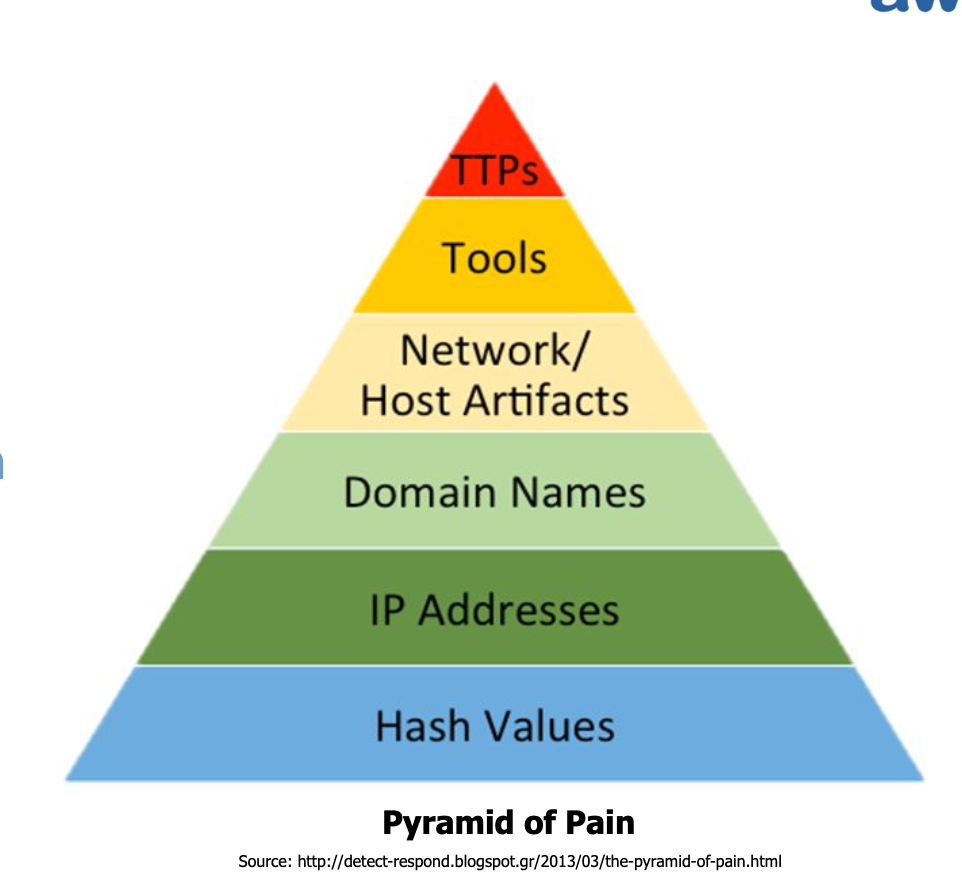
\includegraphics[width=0.4\linewidth]{Figures/pyramid_of_pain.png}
\end{center}

\subsection{Concept -- two separate axes \hl{(!)}}
Detecting \& responding to an indicator fast = \kw{denying the adversary its use}. Each indicator has \kw{two independent properties}:
\begin{itemize}
\item \kw{Accuracy} (good for \kw{you}): if it matches, how sure it's really malicious (few false positives).
\item \kw{Pain} (cost to the \kw{attacker}): how hard/costly to \kw{change it} \& evade you.
\end{itemize}
Bottom = trivial for attacker to change, top = must reinvent. \textit{Ex: a \kw{hash} = high accuracy (matches exactly one file) but \hl{trivial pain} -- attacker flips 1 bit / recompiles $\to$ new hash $\to$ your block is useless $\Rightarrow$ whack-a-mole. A \kw{TTP} = high pain (attacker must change how they operate) but lower accuracy (legit admins also use e.g. PowerShell $\to$ false positives).}

\subsection{Levels (low $\to$ high pain)}
\begin{itemize}
\item \kw{Hash values} -- pain \hl{Trivial}, accuracy High. \textit{Flip 1 bit $\to$ new hash.}
\item \kw{IP addresses} -- pain \hl{Easy}, acc. Med-High. \textit{(Anon) proxies, fast-flux.}
\item \kw{Domain names} -- pain \hl{Simple}, acc. Med-High. \textit{Must register/host, but lax/anon registrars (crypto) make it cheap.}
\item \kw{Network/Host artifacts} -- pain \hl{Annoying}, acc. Med-High. \textit{URI patterns, C2 in protocols, weird User-Agent; registry keys, dropped files. Attacker must find why detected \& fix it.}
\item \kw{Tools} -- pain \hl{Challenging}, acc. High. \textit{Custom protocols, fuzzy hashes. Attacker must build a new tool (costs time/money).}
\item \kw{TTPs} -- pain \hl{Tough!}, acc. Low-High. \textit{How adversary operates (Pass-the-Hash, spear phishing, tailgating). Detecting the behavior forces them to relearn $\to$ give up or reinvent from scratch.}
\end{itemize}
$\Rightarrow$ \hl{Use indicators that cause the most pain whenever possible.} (SIEM/operational $\to$ lower levels; strategic threat intel $\to$ upper levels.)

\end{multicols*}
